%Corps du document :
%\setlength{\parindent}{1cm}    

\section{Structures de données}

Voici la description des structures de données que nous avons utilisées dans le cadre de ce projet :

\subsection{Diagrammes UML détaillés}

\subsubsection{Modèle XML}

\medskip
\begin {center}
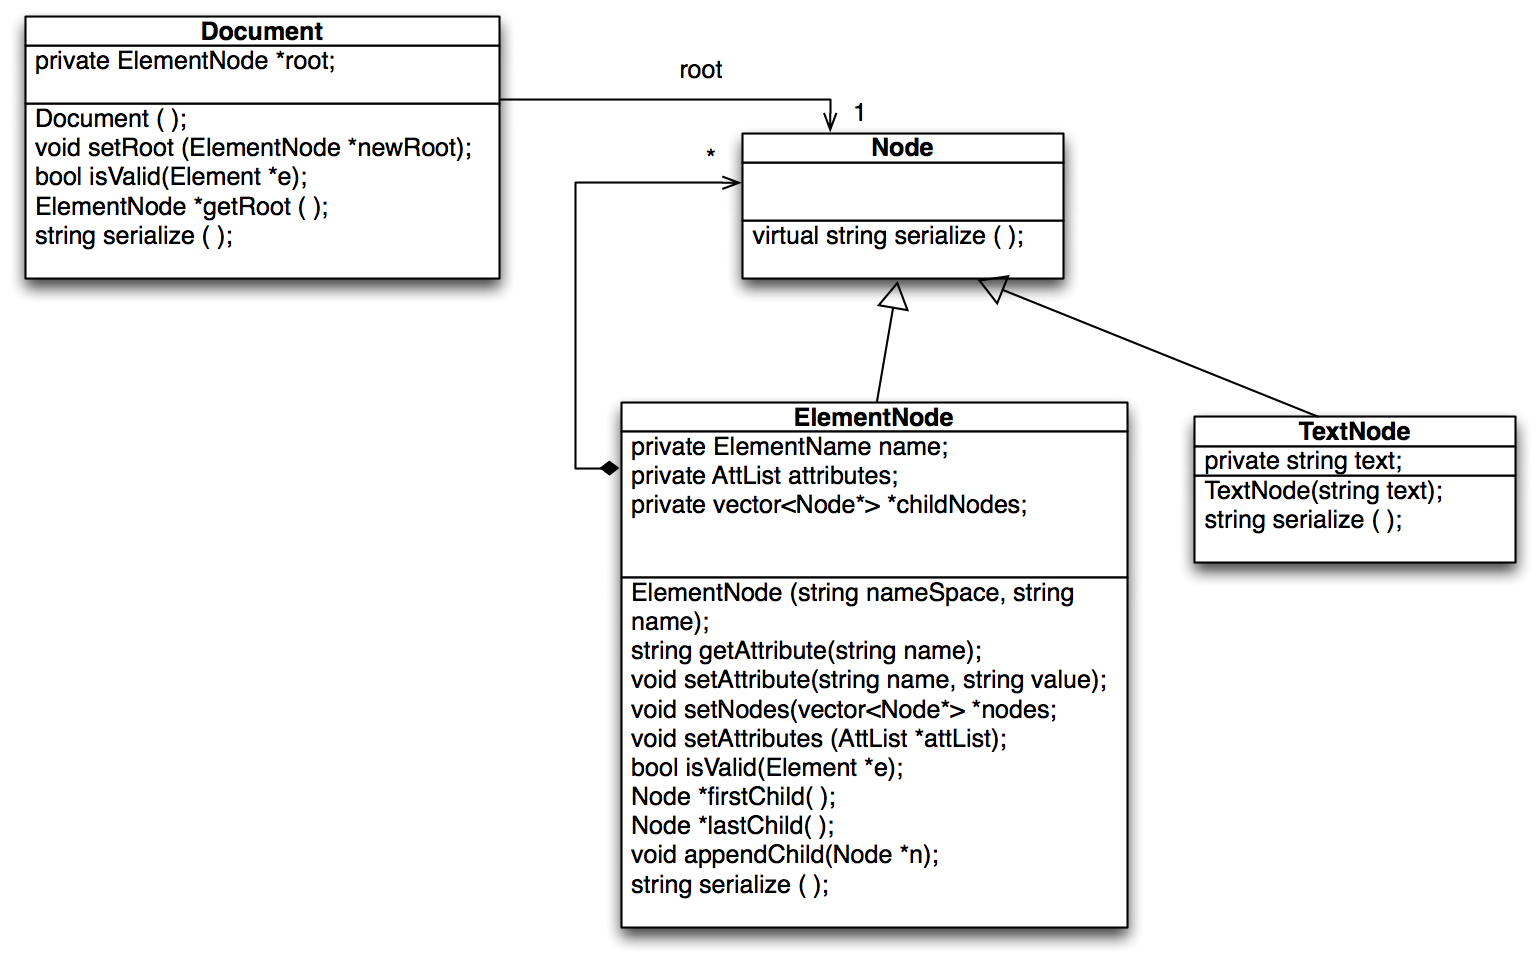
\includegraphics[width=\textwidth]{UMLXML.png}
\end {center}
\medskip

\subsubsection{Modèle DTD}

\medskip
\begin {center}
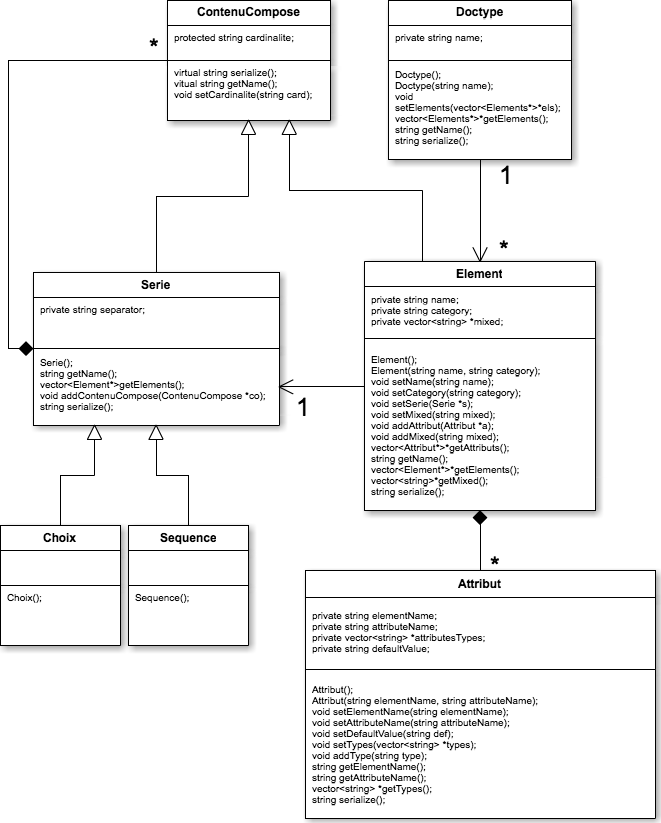
\includegraphics[width=\textwidth]{UMLDTD.png}
\end {center}
\medskip


\section{Algorithmes}

\subsection{Algorithmes de Validation}

\begin{algorithm}
\caption{Document isValid(DocType)}
\begin{algorithmic}
\STATE $sequence \leftarrow new sequence$
\FORALL{$element de DocType$}
\STATE $sequence \leftarrow ajout du contenu composé (element de la DocType)$
\ENDFOR
\STATE $element \leftarrow new Element avec comme serie(sequence)$
\RETURN $nodeDuXML.isValid(element,DocType)$
\end{algorithmic}
\end{algorithm}

\begin{algorithm}
\caption{ElementNode isValid(DocType)}
\begin{algorithmic}
\STATE $LIGNE A CHANGER$
\end{algorithmic}
\end{algorithm}

\subsection{Algorithmes de Transformation}

\begin{algorithm}
\caption{TransformXML(documentXML,documentXSL)}
\begin{algorithmic}
\STATE $resultat \leftarrow new Document$
\FORALL{$template$}
\IF{$template de la raçine$}
\STATE $resultat.racine \leftarrow transformTemplate(templateRacine,elementNode de documentXML$
\ENDIF
\ENDFOR
\RETURN $resultat$
\end{algorithmic}
\end{algorithm}

\begin{algorithm}
\caption{TransformTemplate(nodeXML,template)}
\begin{algorithmic}
\STATE $result \leftarrow liste de node$
\IF{$template n'a pas le namespace xsl$}
\STATE $node \leftarrow new ElementNode(nom de template,attribut de template)$
\STATE $ajout de node dans result$
\ENDIF
\FORALL{$enfant de template$}
\IF{$enfant est un ElementNode$}
\IF{$namespace de l'enfant est xsl$}
\IF{$nom de l'enfant est apply-templates$}
\IF{$un template s'applique à un enfant de nodeXML$}
\STATE $result \leftarrow TransformTemplate(enfant de nodeXML,template à appliquer)$
\ENDIF
\ELSIF{$nom de l'enfant est value-of$}
\STATE $result \leftarrow enfants de nodeXML$
\ENDIF
\ELSE
\STATE $result \leftarrow TransformTemplate(nodeXML,enfant du template)$
\ENDIF
\ELSE
\STATE $result \leftarrow enfant du template$
\ENDIF
\ENDFOR
\RETURN $result$
\end{algorithmic}
\end{algorithm}
